\chapter{Domino Arrangements}

\section{Problem Definition}

\begin{enumerate}
    \item Input:
    \begin{enumerate}
        \item an natural number $n \in \N$;
    \end{enumerate}
    \item Output:
    \begin{enumerate}
        \item a list of all the ways the dominos can be arranged in the $2 \times n$ grid;
    \end{enumerate}
\end{enumerate}

\section{Examples}

\begin{figure}[H]
    \centering
    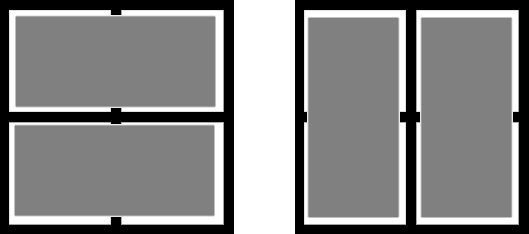
\includegraphics[width=0.4\textwidth]{images/domino_arrangements/2x2_all.png}
    \caption{all arrangments in a $2 \times 2$ grid.}
\end{figure}

\begin{figure}[H]
    \centering
    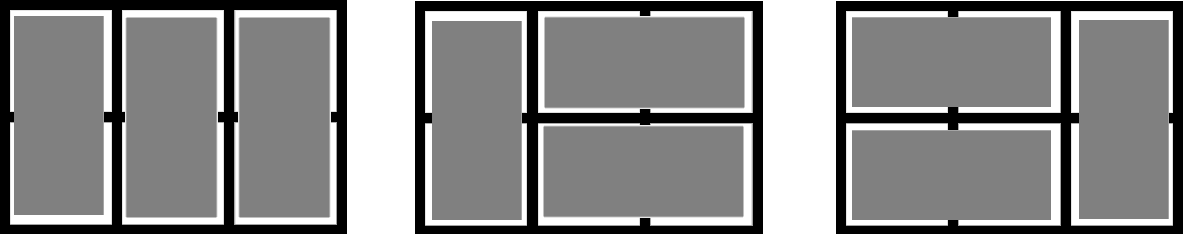
\includegraphics[width=0.7\textwidth]{images/domino_arrangements/2x3_all.png}
    \caption{all arrangments in a $2 \times 3$ grid.}
\end{figure}

\begin{figure}[H]
    \centering
    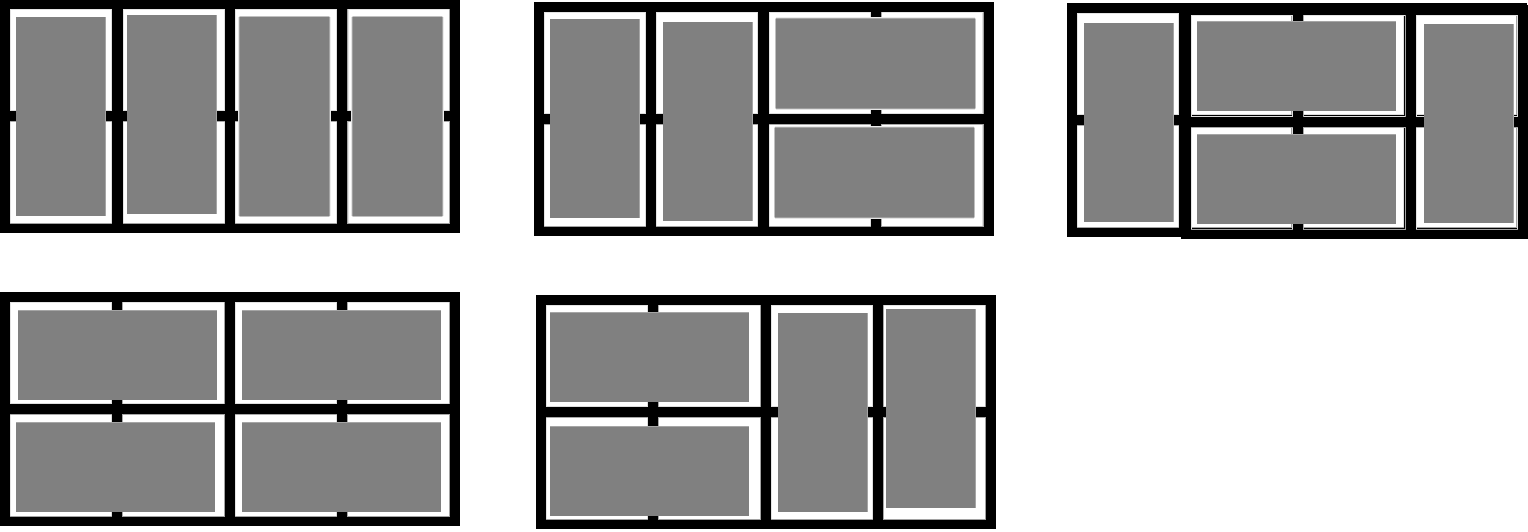
\includegraphics[width=0.9\textwidth]{images/domino_arrangements/2x4_all.png}
    \caption{all arrangments in a $2 \times 4$ grid.}
\end{figure}

\section{Algorithm}

Given $n \in \N$, let $S(n)$ be the solution (all arrangements). $S(n)$ can be obtained from two recursive calls:
\begin{enumerate}
    \item one vertical domino combined with $S(n-1)$;
    \item two horizontal dominos combined with $S(n-2)$;
\end{enumerate}
Such procedure is shown in the Figure

\begin{figure}[H]
    \centering
    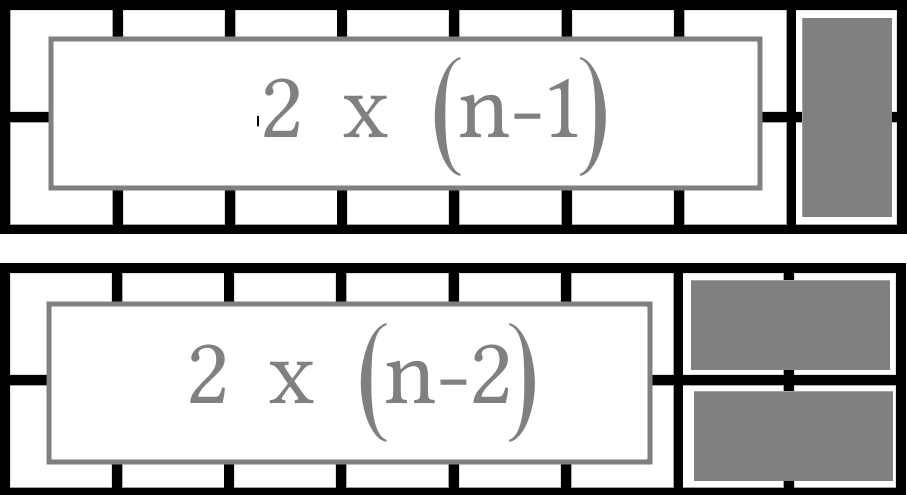
\includegraphics[width=0.7\textwidth]{images/domino_arrangements/2xn_recursive.png}
    \caption{recursive solution for a $2 \times n$ grid.}
\end{figure}

\section{Algorithm}

\begin{figure}[H]
    \centering
    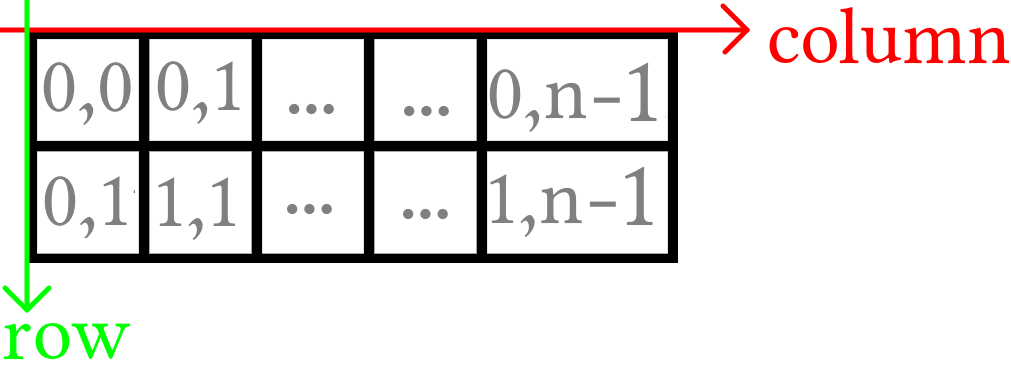
\includegraphics[width=0.9\textwidth]{images/domino_arrangements/grid_cordinates.png}
    \caption{coordinate system for a $2 \times n$ grid.}
\end{figure}

\newcommand{\domino}[2]{\mbox{\textbf{Domino}}\left[\tuple{#1}, vertical\right]}
\newcommand{\dominoV}[1]{\domino{#1}{vertical}}
\newcommand{\dominoH}[1]{\domino{#1}{horizontal}}
\newcommand{\DA}{domino\_arrangements}

\begin{algorithm}[H]
    \caption{\DA}
    \label{domino-arrangements:algorithm}
    \begin{algorithmic}[1]
        \Require{$n \in \N$}
        \If{$n == 1$}
            \State{\textbf{return} $$\Big\langle
                    \tuple{\dominoV{0,0}}
                \Big\rangle$$
            }
            \label{domino-arrangements:algorithm:n=1}
        \ElsIf{$n == 2$}
        \State{\textbf{return} $$\Big\langle
                \tuple{\dominoV{0,0}, \dominoV{0,1}},
            $$$$
                \tuple{\dominoH{0,0}, \dominoH{1,0}}
            \Big\rangle$$
            \label{domino-arrangements:algorithm:n=2}
        }
        \Else
            \State{\textbf{return} $$
                \text{\DA}(n-1) \oplus \tuple{\dominoV{0,0}},
                $$$$
                \text{\DA}(n-2) \oplus \tuple{\dominoH{0,0}, \dominoH{1,0}}
            $$}
            \Comment{$\oplus$ is the concatenation of the list on the right with all the lists on the left.}
        \EndIf
    \end{algorithmic}
\end{algorithm}

\section{Correctness of the Algorithm}

\subsection*{Base Case 1}

By inspection, one notices that for a $2 \times n$ grid, there are two possible arrangements. Therefore, the line \ref{domino-arrangements:algorithm:n=1} of the algorithm returns the optimal solution of the case $n = 1$.

\subsection*{Base Case 2}

By inspection, one notices that for a $2 \times n$ grid, there are two possible arrangements. Therefore, the line \ref{domino-arrangements:algorithm:n=2} of the algorithm returns the optimal solution of the case $n = 2$.

\subsection*{Recursion}

First of all, notice that, if a domino is in the horizontal position, then there must be a domino right over (or below) it. In other words, arrangements such as the one of the Figure \ref{domino-arrangements:figure:impossible-arrangement}.

Now, for the last domino, there is two possibilities: either it is in the vertical or the horizontal (and so there is another one below it) position. But for both cases, the problem of arranging the other dominos is the same problem but with a smaller grid:

\begin{enumerate}
    \item the last domino is in the vertical position: solve the problem for the grid $2 \times (n-1)$
    \item the last domino is in the horizontal position: solve the problem for the grid $2 \times (n-2)$
\end{enumerate}

\begin{figure}[H]
    \centering
    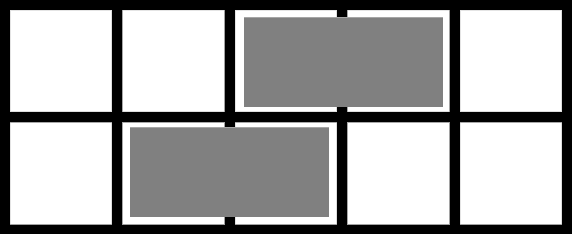
\includegraphics[width=0.6\textwidth]{images/domino_arrangements/2x5_impossible.png}
    \caption{invalid configuration of dominos. A horizontal domino must have another right over or below it.}
    \label{domino-arrangements:figure:impossible-arrangement}
\end{figure}
